\documentclass[pre,twocolumn,superscriptaddress,longbibliography,floatfix]{revtex4-2}
\usepackage{graphicx}
\usepackage{amsmath,amssymb}
\usepackage{bm}
\usepackage{url}
\usepackage[colorlinks=true,linkcolor=blue,citecolor=blue,urlcolor=blue]{hyperref}

\newcommand{\pc}{p_c}
\newcommand{\ps}{p_c^{\rm site}}
\newcommand{\pb}{p_c^{\rm bond}}
\newcommand{\zb}{\bar z}

\begin{document}
\raggedbottom

\title{Site and bond percolation thresholds of all $k$-uniform tilings with $k\le 10$}

\author{Maksim Elisov}
\email{maksimelisov2003@gmail.com}
\homepage{ORCID: 0009-0001-3097-2703}
\affiliation{Samara National Research University, 34 Moskovskoye shosse, Samara 443086, Russia}

\date{\today}

\begin{abstract}
We determine the site and bond percolation thresholds of all 23\,396 $k$-uniform tilings of the plane by regular polygons with $k\le 10$ (the complete set according to the known enumeration), i.e., 46\,792 thresholds. The thresholds are obtained by microcanonical Monte Carlo simulation on tori with the criterion that the probabilities of no wrapping and of a cross-wrapping cluster are equal. Under the standard duality (matching) and universality assumptions this criterion is expected to hold in the scaling limit for every torus shape, so it applies to the many tilings without three-, four-, or sixfold rotations; we validate it numerically. For the 243 tilings with $k\le 4$, including the 61 three-uniform and 151 four-uniform tilings, for which, to our knowledge, no thresholds were previously available, finite-size extrapolation gives uncertainties of a few units in the sixth decimal (median $3\times10^{-6}$); the 22 Archimedean reference values are reproduced with a root-mean-square deviation of 0.82 standard errors. For $k=5$--$10$, single-torus runs give statistical uncertainties of $2$--$7\times10^{-5}$; a check of 200 of these thresholds on larger, near-square tori shows no finite-size bias at this level. The site thresholds of the two-uniform lattices are improved by a factor of about 60, and the value for $\tfrac12(3.12^2)+\tfrac12(3.4.3.12)$ is revised to $0.7671769(30)$. A linear rule in the vertex-type fractions predicts the thresholds of the 23\,153 tilings with $k\ge5$ with an rms error of $2\times10^{-3}$, 2.5 (site) to 7 (bond) times more accurately than the Euler-characteristic estimate and an order of magnitude more accurately than the Galam--Mauger formula; nevertheless, tilings with identical vertex composition differ by up to $6\times10^{-3}$ (site) and $2\times10^{-2}$ (bond). In the minimal case, pairs of tilings that differ only by the registry of strips separated by $h$ rows of squares, the bond threshold difference falls by a factor of 6 to 8 per row, consistent in magnitude with the leading eigenvalue of the square-band transfer matrix in the momentum-$\pi$ sector, $\lambda_\pi\approx0.15$, which suggests a simple mechanism for the decay; the site difference is smaller and changes sign.
\end{abstract}

\maketitle

%=====================================================================
\section{Introduction}
%=====================================================================

The percolation threshold $\pc$ is the simplest lattice-dependent quantity of percolation theory, and the one most often needed in applications~\cite{StaufferAharony,Grimmett99}. In two dimensions exact values are known for a few lattices: $1/2$ for site percolation on the triangular lattice~\cite{Kesten82} and for bond percolation on the square lattice~\cite{Kesten80}, $2\sin(\pi/18)$ and $1-2\sin(\pi/18)$ for bond percolation on the triangular and honeycomb lattices~\cite{SykesEssam64,Wierman81}, and further values that follow from star--triangle and self-duality arguments~\cite{SykesEssam64,ZiffScullard06,ScullardZiff08,WiermanZiff11,GrimmettManolescu14}. For all other lattices $\pc$ is known numerically, from Monte Carlo simulation~\cite{NewmanZiff00,NewmanZiff01,FengDengBlote08}, from critical polynomials and transfer matrices~\cite{ScullardJacobsen12,JacobsenScullard13,Jacobsen14,Jacobsen15,ScullardJacobsen20}, or within rigorous confidence intervals~\cite{RiordanWalters07}.

The tilings of the plane by regular polygons are a natural family of test lattices. A tiling is $k$-uniform if it is edge-to-edge and its vertices form $k$ orbits under its symmetry group~\cite{GrunbaumShephard87}. There are 11 one-uniform (Archimedean) tilings, 20 two-uniform tilings~\cite{GrunbaumShephard87}, 61 three-uniform tilings~\cite{Chavey84,Chavey89}, and the number grows roughly as $2^k$, to 11\,866 at $k=10$; the enumeration is due to Galebach~\cite{Galebach,OEIS_A068599} and was extended by \v{C}trn\'act~\cite{OEIS_A068599,TesCatalog}. Of the 21 possible vertex types, 15 occur in tilings~\cite{GrunbaumShephard87}. Tilings by regular polygons appear as lattices of real materials~\cite{Li22}, as periodic approximants of dodecagonal square--triangle tilings~\cite{OxborrowHenley93}, and as test lattices for spin models~\cite{Yu17}; recently, the meshes of all $k$-uniform tilings with $k\le6$ were edge-colored to construct quantum circuits~\cite{Kattemolle25}. Thresholds of aperiodic tilings are known for the Penrose tiling and for octagonal and dodecagonal quasilattices~\cite{Babalievski95,ZiffBabalievski99}.

The site and bond thresholds of the Archimedean lattices are known to high precision~\cite{SudingZiff99,Parviainen07,FengDengBlote08,Jacobsen14,Jacobsen15,ScullardJacobsen20}. For the 20 two-uniform lattices, Neher, Mecke, and Wagner obtained the site thresholds with an uncertainty of $2\times10^{-4}$~\cite{Neher08,Neher08supp}; we are not aware of a published source for their bond thresholds. We did not find any published thresholds for $k\ge3$ (literature search of 16 October 2026). The many proposed ``universal'' formulas for $\pc$~\cite{ScherZallen70,Vyssotsky61,GalamMauger96,GalamMauger97,GalamMauger98,vanderMarck97,WiermanNaor05,Neher08,Lebrecht21} have been calibrated and tested on a few dozen two-dimensional lattices at most.

In this paper we compute both thresholds of all 23\,396 $k$-uniform tilings with $k\le10$. The 486 thresholds with $k\le4$ have uncertainties of a few units in the sixth decimal, the remaining 46\,306 have statistical uncertainties of $2$--$7\times10^{-5}$. The data set allows a quantitative look at two old questions: how well $\pc$ can be predicted from local information, and how strongly it depends on the arrangement of a given set of vertex types. We find that rules based on the vertex composition alone predict $\pc$ to about $2\times10^{-3}$, while the arrangement shifts $\pc$ by up to $2\times10^{-2}$. The smallest arrangement change, a slip of strips by half a period, gives threshold differences that decay exponentially with the distance between the strips, at a rate consistent with a transfer-matrix estimate.

The paper is organized as follows. Section~\ref{sec:tilings} describes the conversion of the tiling catalog into periodic graphs. Section~\ref{sec:method} describes the simulations, the threshold estimator, and its validation. Section~\ref{sec:results} presents the thresholds and tests empirical rules. Section~\ref{sec:slip} analyzes the slip pairs, and Sec.~\ref{sec:concl} concludes. Appendix~\ref{app:tm} gives the transfer-matrix details and Appendix~\ref{app:tab} lists the thresholds of the 61 three-uniform tilings. The thresholds of all tilings are given in the Supplemental Material~\cite{SM}.

%=====================================================================
\section{Tilings and periodic graphs}\label{sec:tilings}
%=====================================================================

\begin{figure*}
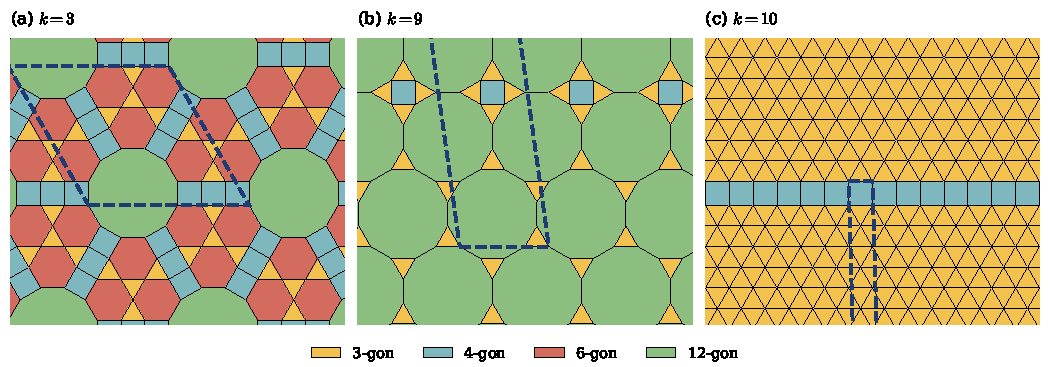
\includegraphics[width=\textwidth]{figs/fig_examples.pdf}
\caption{Examples of $k$-uniform tilings; the dashed parallelograms are unit cells. (a) A three-uniform tiling with vertex types $\tfrac25(3.4^2.6)+\tfrac25(4.6.12)+\tfrac15(3.6.3.6)$, $\ps=0.6857748(35)$, $\pb=0.5911238(28)$. (b) The tiling with the highest site and bond thresholds among the non-Archimedean tilings with $k\le10$, $\tfrac{11}{13}(3.12^2)+\tfrac{2}{13}(3.4.3.12)$ ($k=9$), $\ps=0.79687(5)$, $\pb=0.72270(6)$. (c) The tiling with the lowest non-Archimedean thresholds, $\tfrac{9}{10}(3^6)+\tfrac{1}{10}(3^3.4^2)$ ($k=10$), $\ps=0.50535(7)$, $\pb=0.35441(6)$: one row of squares in every twenty rows of polygons.}
\label{fig:examples}
\end{figure*}

We take the tilings from the tessellation catalog of \v{C}trn\'act and Kopczy\'nski~\cite{TesCatalog}, which contains, among other tilings, all $k$-uniform tilings with $k\le10$. The numbers of tilings, 11, 20, 61, 151, 332, 673, 1472, 2850, 5960, and 11\,866 for $k=1,\dots,10$, agree with the known enumeration~\cite{OEIS_A068599}; the completeness of our set for $k\ge8$ rests on that enumeration. Each catalog file specifies the polygons, the gluing of their edges, and the vertex type of every vertex orbit.

From each file we construct a periodic graph. A patch of polygons is laid out by breadth-first gluing; the translation lattice is found by testing, in order of increasing length, the vectors from a vertex to the other vertices of the same type, a vector being accepted if it maps the patch onto itself; the basis is Lagrange--Gauss reduced to $(\mathbf T_1,\mathbf T_2)$ with $|\mathbf T_1|\le|\mathbf T_2|$; and the vertices are identified modulo translations. The result is a cell with $n_v$ vertices and a list of $n_e$ edges $(u,w,a,b)$, each joining vertex $u$ of cell $(0,0)$ to vertex $w$ of cell $(a,b)$. We checked for every tiling that the Euler characteristic of the cell vanishes, $n_v-n_e+n_f=0$, and that the vertex types found in the cell are those of the catalog. For $k\le4$ we also computed the full symmetry group of the patch and checked that the vertices form exactly $k$ orbits. All 23\,396 tilings pass these checks. Figure~\ref{fig:examples} shows three examples.

We label vertex types by the cyclic sequence of polygons around a vertex~\cite{GrunbaumShephard87}, e.g., $(3.4^2.6)$ for triangle, square, square, hexagon, and a tiling by its composition, the fractions of vertices of each type; for instance $\tfrac45(3.4^2.6)+\tfrac15(3.6.3.6)$ is the composition of two different two-uniform tilings. Of the 243 tilings with $k\le4$, 147 have no rotation of order 3, 4, or 6; such lattices need not be isotropic at large scales. The share of such tilings grows with $k$, and the unit cells reach $n_v=120$ vertices at $k=10$.

\begin{table}
\caption{Number of $k$-uniform tilings, the protocol, and the median uncertainty of the site and bond thresholds (in units of $10^{-6}$). For $k\le4$: error of the finite-size extrapolation (statistical); changing the correction exponent shifts the values by a median of $0.1\sigma$. For $k\ge5$: statistical error; the finite-size bias is below $0.13\sigma$ (95\% bound, Sec.~\ref{sec:method}).}
\label{tab:counts}
\begin{ruledtabular}
\begin{tabular}{rrlrr}
$k$ & tilings & tori & $\sigma_{\rm site}$ & $\sigma_{\rm bond}$\\
\hline
1 & 11 & 3 tori, extrap. & 3.3 & 2.6 \\
2 & 20 & 3 tori, extrap. & 3.5 & 2.6 \\
3 & 61 & 3 tori, extrap. & 3.5 & 2.7 \\
4 & 151 & 3 tori, extrap. & 2.9 & 2.4 \\
5 & 332 & 1 torus & 21.4 & 18.4 \\
6 & 673 & 1 torus & 21.4 & 18.5 \\
7 & 1472 & 1 torus & 22.9 & 19.9 \\
8 & 2850 & 1 torus & 63.0 & 55.6 \\
9 & 5960 & 1 torus & 64.4 & 57.9 \\
10 & 11866 & 1 torus & 74.9 & 68.6 \\

\end{tabular}
\end{ruledtabular}
\end{table}

%=====================================================================
\section{Method}\label{sec:method}
%=====================================================================

\subsection{Simulation}

We use the microcanonical algorithm of Newman and Ziff~\cite{NewmanZiff00,NewmanZiff01} on tori of $L_x\times L_y$ unit cells. In each sample the $N$ sites (or bonds) of the torus are occupied one by one in a uniformly random order, and clusters are maintained by union--find with path compression. Every element stores its displacement to its parent, so that when an occupied element closes a cycle within a cluster, the winding vector of the cycle is obtained at no extra cost~\cite{NewmanZiff01}. For each sample we record the number of occupied elements $n_e$ at which a cluster first wraps the torus in any direction, and the number $n_x$ at which a single cluster first acquires two independent winding vectors (a cross configuration); the sample stops at $n_x$. The canonical probabilities follow by the exact binomial convolution,
\begin{equation}
R_X(p)=\frac1M\sum_{j=1}^{M}\Pr\!\left[\mathrm{Bin}(N,p)\ge n_X^{(j)}\right],\quad X=e,x,
\end{equation}
where $M$ is the number of samples. The statistical errors of $R_X(p)$ follow from the variance of the summands, so no binning is needed. Random numbers are generated by xoshiro256** (sequential code) or xoshiro128** (data-parallel code), seeded through splitmix64 from a hash of the run name, with distinct streams for all parallel runs. The two codes give identical histograms when run on identical random-number streams.

\subsection{Threshold estimator}

Let $P_0(p)=1-R_e(p)$ be the probability that no cluster wraps the torus and $P_+(p)=R_x(p)$ the probability of a cross configuration. Under planar duality (bond percolation) or matching (site percolation), a configuration without a wrapping cluster corresponds to a complementary configuration that contains a cross cluster, and vice versa~\cite{MertensZiff16}. Hence $P_0(p)=P_+^\ast(1-p)$, where the star denotes the dual (matching) model. Assuming universality, i.e., that the critical model and its dual (matching) partner have the same conformally invariant scaling limit on the same torus (proven for site percolation on the triangular lattice), $P_0=P_+$ at $\pc$ in the scaling limit for every torus modular parameter $\tau$. Pinson derived this equality, $\pi(\mathbb Z\times\mathbb Z)=\pi(0)$, by the same duality argument when computing the wrapping probabilities of critical percolation on the torus~\cite{Pinson94}, and Arguin gave the corresponding relation for the Potts model~\cite{Arguin02}; see also Refs.~\cite{DiFrancesco87,ZiffLorenzKleban99}. We checked it numerically with Pinson's expressions for square and rhombic tori. We therefore define the finite-size estimate $p_N$ as the root of
\begin{equation}
R_e(p)+R_x(p)=1.
\label{eq:cross}
\end{equation}
The status of the ingredients is as follows. The complementarity of no-wrapping and cross configurations under duality or matching is an exact topological statement on every finite torus~\cite{MertensZiff16}. The equality $P_0=P_+$ at $\pc$ on a general torus additionally requires that the critical model and its dual (matching) partner have the same conformally invariant scaling limit; this universality is proven only for site percolation on the triangular lattice~\cite{Smirnov01} and is otherwise an assumption, which we test numerically below (Sec.~\ref{sec:valid}), including the anisotropic lattice $(3^3.4^2)$. Since every summand of $R_e$ and $R_x$ is a nondecreasing function of $p$, $R_e+R_x$ is strictly increasing, so Eq.~\eqref{eq:cross} has exactly one root on every finite torus; we locate it by Brent's method on a bracket with a sign change.
This is the Monte Carlo counterpart of the critical polynomial of Jacobsen and Scullard, $P_B(p)=P_{2D}(p)-P_0(p)$, whose roots converge to $\pc$ very rapidly~\cite{JacobsenScullard13,Jacobsen14}; Mertens and Ziff derived the underlying topological identities for finite matching lattices from Euler's formula~\cite{MertensZiff16}. In contrast to the common criterion $R_e(p)=R_e^\infty(\tau)$, Eq.~\eqref{eq:cross} needs no knowledge of the universal value $R_e^\infty(\tau)$. This is essential here: for a lattice without three-, four-, or sixfold rotations, the effective modular parameter of the critical torus may differ from the geometric one by an unknown anisotropy, and $R_e^\infty$ is then not known. For the uncertainty of $p_N$ we use $(\sigma_e+\sigma_x)/|d(R_e+R_x)/dp|$, where $\sigma_X$ is the standard error of $R_X(p_N)$ and the derivative is the central finite difference of the exact convolution, with step $2\times10^{-3}/\sqrt N$; its own statistical error is negligible. This is an upper bound for any correlation of $R_e$ and $R_x$; the histograms do not record the joint distribution of $n_e$ and $n_x$, so the exact variance is not available. The comparisons below show that the bound overestimates the errors by about 10--20\%.

\subsection{Finite-size corrections}

For the estimator $R_e(p)=R_e^\infty$ the leading finite-size correction scales as $L^{-2-1/\nu}=L^{-11/4}$~\cite{NewmanZiff00,NewmanZiff01}, while the roots of the exactly computed critical polynomials converge empirically as $L^{-w}$ with $w\approx4$~\cite{MertensZiff16}. We use the slower law $L^{-11/4}$ and check below that the results are insensitive to this choice. For $k\le4$ (the ``core'') we simulated three tori per threshold, with $L_x|\mathbf T_1|\approx L_y|\mathbf T_2|$ (aspect ratios 0.87--1.15) and median sizes of 504, 2016, and 8100 sites, and fitted
\begin{equation}
p_N=\pc+aN^{-11/8},
\label{eq:fss}
\end{equation}
with $N$ the number of sites (also for bond percolation, where the number of bonds is proportional to $N$). The fits have one degree of freedom; the median $\chi^2$ is 0.37 and 2.7\% of the fits exceed the 95\% point 3.84. The quoted errors are the fit errors, not rescaled by $\chi^2$. Changing the exponent from $11/4$ to $4$ changes $\pc$ by a median of $0.10\sigma$ and at most $0.81\sigma$; with exponents between 2 and 5 the changes stay below $1.2\sigma$ (median $\le0.14\sigma$). The median number of samples is $1.3\times10^8$ per threshold, $7.5\times10^{10}$ in total.

For $k=5$--10 (the ``atlas'') each threshold comes from a single torus with $N\ge738$ sites (median 1024 for $k=5$, 1764 for $k=10$). For many tilings with long unit cells this torus is elongated: 16\% of the atlas tori have an aspect ratio below 1/2 (minimum 0.35). The runs for $k=5$--7 were made in two independent rounds on the same tori; the two rounds agree with an rms deviation of $0.88$ combined standard errors over 4954 thresholds, which confirms the statistical errors. In total the atlas used $1.4\times10^{10}$ samples. The atlas values carry no finite-size correction, and their quoted errors, $2\times10^{-5}$ ($k\le7$) and $(5.6$--$7.5)\times10^{-5}$ ($k\ge8$), are statistical. The amplitudes $a$ fitted in the core suggest that the residual bias is smaller: at $N=1000$, $|a|N^{-11/8}$ is below $4.5\times10^{-6}$ for 90\% and below $1.6\times10^{-5}$ for 99\% of the 486 core thresholds. Since the atlas contains larger cells ($n_v$ up to 120) and more elongated tori than the core, we checked the bias directly on a stratified sample of 100 atlas tilings: the 35 with the most elongated tori (all with aspect ratio 0.35--0.36), the 35 with the largest cells ($n_v=102$--120), and 5 random tilings for each $k=5,\dots,10$. For each of these 200 thresholds we extended the run on the atlas torus and simulated a near-square torus with 3.7--4.6 times as many sites ($7.5\times10^8$ additional samples in total, $3.8\times10^6$ per threshold on average). The extension runs are independent of the original atlas runs; for the 170 thresholds with $k=8$--10, where the atlas has only one round, they agree with the atlas values with an rms deviation of 0.82 combined standard errors (no deviation above $3\sigma$), which confirms the statistical errors also for $k\ge8$. The difference $\Delta=p_{N_2}-p_{N_1}$ between the larger and the atlas torus measures the finite-size bias of the atlas value (up to a factor $1-(N_2/N_1)^{-\omega/2}\approx0.85$--0.94); its uncertainty is about half the atlas error. We find $\langle\Delta/\sigma_\Delta\rangle=-0.01$ and an rms of 0.94, with no $|\Delta|>3\sigma_\Delta$; the largest $|\Delta|$ is 1.75 atlas standard errors. The rms of $\Delta/\sigma_\Delta$ is between 0.87 and 1.00 in every subgroup ($k=5$--7 and 8--10, aspect ratio below and above 1/2, $n_v$ below and above 100), and the subgroup means lie between $-0.21$ and $+0.10$. Subtracting the statistical variance, the rms bias is consistent with zero, with a 95\% upper bound of 0.13 atlas standard errors (0.18 for the elongated tori, 0.27 for the largest cells, 0.24 for the random sample). Within the precision of the atlas, its values are therefore free of finite-size bias. The check runs are listed in the Supplemental Material~\cite{SM}.

Figure~\ref{fig:validation}(b) shows the finite-size behavior directly for eight Archimedean thresholds, simulated on tori of 54 to 1058 sites with $\sigma\approx3\times10^{-6}$ each. For seven of them no deviation from the exact or high-precision value is visible even on the smallest tori. The site threshold of the square lattice is the exception: $p_N-\pc=-108$, $-34$, and $-9\times10^{-6}$ for $N=64$, 121, and 256, and zero within errors for $N\ge529$. In the core fits no finite-size amplitude is significant at the $3\sigma$ level.

\begin{figure*}
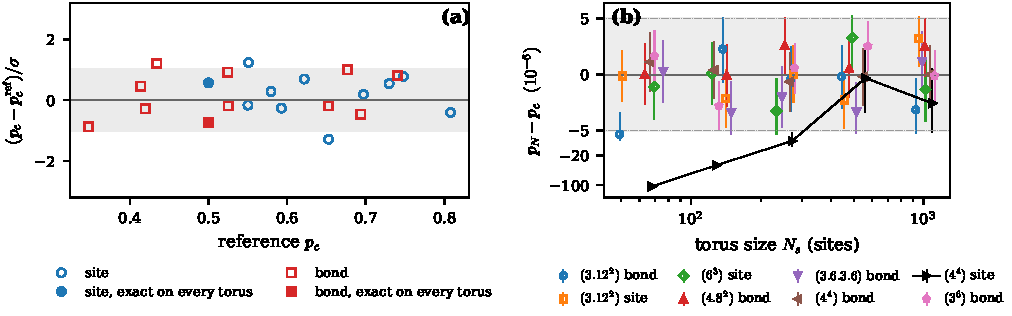
\includegraphics[width=\textwidth]{figs/fig_validation.pdf}
\caption{(a) Deviation of our thresholds from the 22 Archimedean reference values (exact values and Refs.~\cite{SudingZiff99,Jacobsen14,Jacobsen15,ScullardJacobsen20}) in units of the combined standard error. Filled symbols: the two thresholds that are exact on every finite torus by self-matching or self-duality, $\ps(3^6)$ and $\pb(4^4)$; they test the statistical errors only. The shaded band is $\pm1\sigma$. (b) Finite-size estimates $p_N$ of Eq.~\eqref{eq:cross} minus the reference value for eight Archimedean thresholds, as a function of the torus size. Only the square-lattice site threshold (connected symbols) shows a visible correction.}
\label{fig:validation}
\end{figure*}

\subsection{Validation}\label{sec:valid}

Table~\ref{tab:arch} and Fig.~\ref{fig:validation}(a) compare our values with the 22 Archimedean thresholds. The deviation is $+0.22\sigma$ on average and $0.82\sigma$ rms, with a maximum of $2.3\sigma$; without the two thresholds that are exact on every finite torus, the rms deviation is $0.83\sigma$. The error bars are thus realistic, if slightly conservative. The largest deviation is for the site threshold of $(3^2.4.3.4)$, where we find $0.5508171(38)$ against $0.550806(3)$ from Ref.~\cite{SudingZiff99}. Our values for $(3^4.6)$ and $(3^3.4^2)$, the other two site thresholds known only to this precision, agree with Ref.~\cite{SudingZiff99}. For comparison, the values of Ref.~\cite{SudingZiff99} for $(3.4.6.4)$ and $(4.6.12)$ differ from the later high-precision values~\cite{Jacobsen14} by $2.3$ and $1.3$ times their quoted uncertainty, so a deviation of this size is not unusual. The reference set contains no high-precision site threshold of a lattice with more than one vertex orbit.

\begin{table*}
\caption{Archimedean lattices: our thresholds, the reference values, and the deviation $z=(\pc-p_c^{\rm ref})/\sigma$ in units of the combined standard error. Reference values written with ``\ldots'' are exact or known to more digits than shown; $\dagger$: exact on every finite torus.}
\label{tab:arch}
\begin{ruledtabular}
\begin{tabular}{lllrllr}
lattice & $\ps$ (this work) & $\ps$ (reference) & $z$ & $\pb$ (this work) & $\pb$ (reference) & $z$\\
\hline
$(3.12^{2})$ & 0.8078999(22) & 0.807900764\ldots~\cite{SudingZiff99} & -0.4 & 0.7404231(29) & 0.7404207989\ldots~\cite{ScullardJacobsen20} & +0.8 \\
$(4.6.12)$ & 0.7478030(28) & 0.7478008(2)~\cite{Jacobsen14} & +0.8 & 0.6937319(26) & 0.6937331249\ldots~\cite{ScullardJacobsen20} & -0.5 \\
$(4.8^{2})$ & 0.7297248(29) & 0.7297232(5)~\cite{Jacobsen14} & +0.5 & 0.6768058(26) & 0.6768031244\ldots~\cite{ScullardJacobsen20} & +1.0 \\
$(6^{3})$ & 0.6970408(30) & 0.697040230(5)~\cite{Jacobsen14} & +0.2 & 0.6527031(27) & 0.652703645\ldots~\cite{SykesEssam64} & -0.2 \\
$(3.6.3.6)$ & 0.6526994(33) & 0.652703645\ldots~\cite{SykesEssam64} & -1.3 & 0.5244075(27) & 0.5244049992\ldots~\cite{ScullardJacobsen20} & +0.9 \\
$(3.4.6.4)$ & 0.6218145(35) & 0.62181207(7)~\cite{Jacobsen14} & +0.7 & 0.5248310(27) & 0.5248314616\ldots~\cite{ScullardJacobsen20} & -0.2 \\
$(4^{4})$ & 0.5927452(33) & 0.5927460508\ldots~\cite{Jacobsen15} & -0.3 & 0.4999981(26) & 1/2~\cite{Kesten80}$^{\dagger}$ & -0.7 \\
$(3^{4}.6)$ & 0.5794994(38) & 0.579498(3)~\cite{SudingZiff99} & +0.3 & 0.4343316(27) & 0.4343283172\ldots~\cite{ScullardJacobsen20} & +1.2 \\
$(3^{2}.4.3.4)$ & 0.5508171(38) & 0.550806(3)~\cite{SudingZiff99} & +2.3 & 0.4141390(24) & 0.4141378566\ldots~\cite{ScullardJacobsen20} & +0.5 \\
$(3^{3}.4^{2})$ & 0.5502122(38) & 0.550213(3)~\cite{SudingZiff99} & -0.2 & 0.4196396(25) & 0.4196403589\ldots~\cite{ScullardJacobsen20} & -0.3 \\
$(3^{6})$ & 0.5000021(36) & 1/2~\cite{SykesEssam64}$^{\dagger}$ & +0.6 & 0.3472945(22) & 0.347296355\ldots~\cite{SykesEssam64} & -0.9 \\

\end{tabular}
\end{ruledtabular}
\end{table*}

%=====================================================================
\section{Results}\label{sec:results}
%=====================================================================

\subsection{Two-, three-, and four-uniform tilings}

\begin{table*}
\caption{Two-uniform lattices, ordered by decreasing site threshold. ID: catalog file name~\cite{TesCatalog}. Site thresholds are compared with Neher \textit{et al.}~\cite{Neher08supp}. $^\ast$The two lattices with composition $\tfrac45(3.4^2.6)+\tfrac15(3.6.3.6)$ differ in the registry of their strips (Sec.~\ref{sec:slip}); Ref.~\cite{Neher08supp} lists two values for this composition without identifying the lattices.}
\label{tab:2uni}
\begin{ruledtabular}
\begin{tabular}{lllll}
ID & vertex types & $\ps$ (this work) & $\ps$~\cite{Neher08supp} & $\pb$ (this work)\\
\hline
\texttt{3a 4b 1} & $\tfrac{1}{2}(3.12^{2})+\tfrac{1}{2}(3.4.3.12)$ & 0.7671769(30) & 0.7680(2) & 0.6749333(29) & 0.6749 \\
\texttt{3c 4l 1} & $\tfrac{2}{3}(4.6.12)+\tfrac{1}{3}(3.4.6.4)$ & 0.7154422(31) & 0.7157(2) & 0.6453683(25) & 0.6454 \\
\texttt{4a 6d 1} & $\tfrac{6}{7}(3^{2}.4.12)+\tfrac{1}{7}(3^{6})$ & 0.6806338(34) & 0.6808(2) & 0.5577774(29) & 0.5578 \\
\texttt{4d 4f 1} & $\tfrac{2}{3}(3^{2}.6^{2})+\tfrac{1}{3}(3.6.3.6)$ & 0.6496372(35) & 0.6499(2) & 0.5363209(27) & 0.5363 \\
\texttt{4d 6a 1} & $\tfrac{6}{7}(3^{2}.6^{2})+\tfrac{1}{7}(3^{6})$ & 0.6332093(44) & 0.6329(2) & 0.5170775(29) & 0.5171 \\
\texttt{4f 4k 2 (eclipsed)} & $\tfrac{4}{5}(3.4^{2}.6)+\tfrac{1}{5}(3.6.3.6)$ & 0.6283846(37) & 0.6286(2)$^{\ast}$ & 0.5189135(26) & 0.5189 \\
\texttt{4f 4k 1 (staggered)} & $\tfrac{4}{5}(3.4^{2}.6)+\tfrac{1}{5}(3.6.3.6)$ & 0.6281115(39) & 0.6279(2)$^{\ast}$ & 0.5176952(27) & 0.5177 \\
\texttt{4k 4l 1} & $\tfrac{2}{3}(3.4^{2}.6)+\tfrac{1}{3}(3.4.6.4)$ & 0.6218435(33) & 0.6221(2) & 0.5197407(26) & 0.5197 \\
\texttt{4d 5a 1} & $\tfrac{1}{2}(3^{4}.6)+\tfrac{1}{2}(3^{2}.6^{2})$ & 0.6169704(45) & 0.6171(2) & 0.4892140(29) & 0.4892 \\
\texttt{4l 5e 1} & $\tfrac{1}{2}(3^{2}.4.3.4)+\tfrac{1}{2}(3.4.6.4)$ & 0.5881281(37) & 0.5883(2) & 0.4657312(26) & 0.4657 \\
\texttt{4l 5c 1} & $\tfrac{1}{2}(3^{3}.4^{2})+\tfrac{1}{2}(3.4.6.4)$ & 0.5880904(35) & 0.5885(2) & 0.4722908(27) & 0.4723 \\
\texttt{4s 5c 1} & $\tfrac{1}{2}(3^{3}.4^{2})+\tfrac{1}{2}(4^{4})$ & 0.5717644(37) & 0.5720(2) & 0.4584432(28) & 0.4584 \\
\texttt{4p 5c 1} & $\tfrac{2}{3}(3^{3}.4^{2})+\tfrac{1}{3}(4^{4})$ & 0.5646310(36) & 0.5648(2) & 0.4452838(25) & 0.4453 \\
\texttt{5a 6d 1} & $\tfrac{3}{4}(3^{4}.6)+\tfrac{1}{4}(3^{6})$ & 0.5605459(36) & 0.5607(2) & 0.4111037(26) & 0.4111 \\
\texttt{5c 5f 1} & $\tfrac{2}{3}(3^{2}.4.3.4)+\tfrac{1}{3}(3^{3}.4^{2})$ & 0.5505125(30) & 0.5504(2) & 0.4154916(22) & 0.4155 \\
\texttt{5d 5f 1} & $\tfrac{1}{2}(3^{3}.4^{2})+\tfrac{1}{2}(3^{2}.4.3.4)$ & 0.5504255(31) & 0.5505(2) & 0.4162784(28) & 0.4163 \\
\texttt{5e 6a 1} & $\tfrac{6}{7}(3^{2}.4.3.4)+\tfrac{1}{7}(3^{6})$ & 0.5440521(35) & 0.5440(2) & 0.4037930(25) & 0.4038 \\
\texttt{5b 6j 1} & $\tfrac{1}{2}(3^{6})+\tfrac{1}{2}(3^{4}.6)$ & 0.5408655(34) & 0.5407(2) & 0.3891478(21) & 0.3891 \\
\texttt{5c 6f 1} & $\tfrac{2}{3}(3^{3}.4^{2})+\tfrac{1}{3}(3^{6})$ & 0.5342744(34) & 0.5342(2) & 0.3949216(26) & 0.3949 \\
\texttt{5c 6i 1} & $\tfrac{1}{2}(3^{6})+\tfrac{1}{2}(3^{3}.4^{2})$ & 0.5260067(28) & 0.5258(2) & 0.3828495(20) & 0.3829 \\

\end{tabular}
\end{ruledtabular}
\end{table*}

Table~\ref{tab:2uni} lists the two-uniform thresholds. For the 18 lattices that can be matched unambiguously, the site thresholds of Neher \textit{et al.}~\cite{Neher08supp} deviate from ours by $2.8\times10^{-4}$ rms; 10 of the 18 values lie within the quoted uncertainty of $2\times10^{-4}$ and 16 within twice that, which suggests that the quoted uncertainty is somewhat underestimated. The largest deviation is for $\tfrac12(3.12^2)+\tfrac12(3.4.3.12)$, the only two-uniform tiling with this composition: we find $0.7671769(30)$ instead of $0.7680(2)$, a difference of $4.1$ quoted standard errors. Our uncertainties are smaller by a factor of about 60. The two tilings with composition $\tfrac45(3.4^2.6)+\tfrac15(3.6.3.6)$ have site thresholds $0.6283846(37)$ (eclipsed) and $0.6281115(39)$ (staggered); their difference, $2.73(5)\times10^{-4}$, is smaller than the difference $7(3)\times10^{-4}$ of the two values of Ref.~\cite{Neher08supp}. We are not aware of a published source for the bond thresholds of the two-uniform lattices.

The thresholds of the 61 three-uniform tilings are given in Tables~\ref{tab:3uni} and \ref{tab:3unib} (Appendix~\ref{app:tab}); those of the 151 four-uniform tilings are in the Supplemental Material~\cite{SM}. The site thresholds of the three-uniform tilings range from 0.517541 to 0.729771 and the bond thresholds from 0.370944 to 0.633689; for $k=4$ the ranges are 0.513227--0.787193 and 0.365030--0.707756.

Through exact duality and matching relations, the thresholds also give those of related lattices: $1-\pb$ is the bond threshold of the dual tiling and $1-\ps$ the site threshold of the matching graph, obtained by joining all vertices of every face. For site percolation the matching relation $\ps(G)+\ps(G^\ast)=1$ is a theorem for all quasi-transitive planar graphs~\cite{GrimmettLi24hyperbolic}, hence for all our tilings. For bond percolation the duality relation is expected on the same grounds~\cite{SykesEssam64}, but the classical proof~\cite{Kesten82} assumes a reflection symmetry that many of our tilings lack~\cite{WiermanZiff11}.

\subsection{All tilings with $k\le10$}

\begin{figure*}
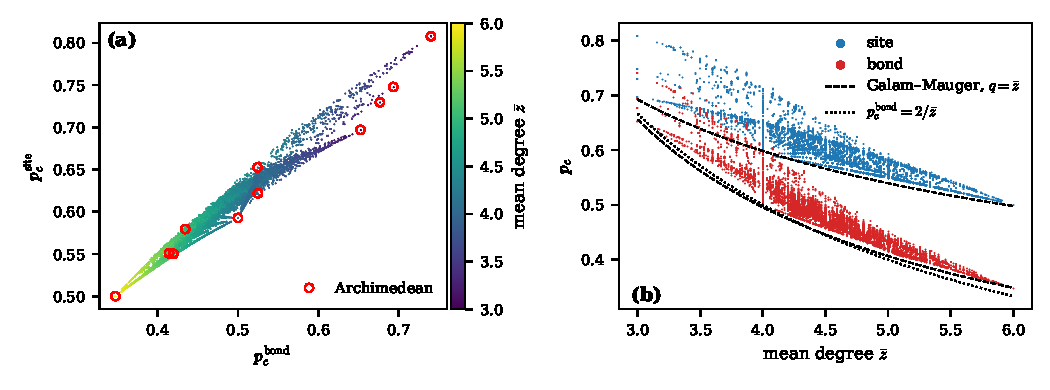
\includegraphics[width=\textwidth]{figs/fig_atlas.pdf}
\caption{(a) Site versus bond threshold for all 23\,396 tilings with $k\le10$, colored by the mean degree $\zb$; circles mark the Archimedean lattices. (b) Site (blue) and bond (red) thresholds versus $\zb$, with the Galam--Mauger formula~\cite{GalamMauger96} evaluated at $q=\zb$ (dashed) and the rule $\pb=2/\zb$~\cite{Vyssotsky61} (dotted). The vertical streaks, e.g., at $\zb=4$ and 5, are tilings with a single vertex degree.}
\label{fig:atlas}
\end{figure*}

Figure~\ref{fig:atlas} gives an overview of all 46\,792 thresholds. All of them lie between the Archimedean extremes: $\tfrac12\le\ps\le0.807901$, attained by $(3^6)$ and $(3.12^2)$, and $0.347296\le\pb\le0.740421$, attained by the same two lattices. The lower bound on $\ps$ is rigorous: the matching graph $G^\ast$ contains the tiling $G$, so $\ps(G^\ast)\le\ps(G)$, and $\ps(G)+\ps(G^\ast)=1$~\cite{GrimmettLi24hyperbolic}. Strict inequality is proven for the transitive (Archimedean) non-triangular tilings~\cite{GrimmettLi24matching}; for the others it is numerical, $\ps-\tfrac12\ge5.3\times10^{-3}$ (72 standard errors) for every tiling except $(3^6)$. The non-Archimedean tilings closest to the bounds are shown in Fig.~\ref{fig:examples}: the triangular lattice with one row of squares in every twenty rows, $\ps=0.50535(7)$, and the $(3.12^2)$ lattice interrupted by rows of $(3.4.3.12)$ vertices, $\ps=0.79687(5)$. The same two tilings also have the extreme non-Archimedean bond thresholds. The site and bond thresholds are strongly correlated (correlation coefficient 0.978), but at a fixed bond threshold the site threshold varies by up to 0.05, as the band structure of Fig.~\ref{fig:atlas}(a) shows.

\subsection{Empirical rules}

\begin{table*}
\caption{Accuracy of empirical rules: rms of the estimate minus the threshold on the hold-out tilings with $k\ge5$. ``A'': the 6504 tilings whose vertex types all occur in Archimedean lattices, where Eq.~\eqref{eq:avg} is defined; ``all'': all 23\,153 tilings with $k\ge5$. The column ``fitted'' gives the number of parameters fitted on the 243 tilings with $k\le4$ (zero for rules taken as published). The last two rows predict $\ps$ from the measured $\pb$.}
\label{tab:rules}
\begin{ruledtabular}
\begin{tabular}{lrllll}
 & & \multicolumn{2}{c}{site} & \multicolumn{2}{c}{bond}\\
rule & fitted & A & all & A & all\\
\hline
Galam--Mauger~\cite{GalamMauger96}, $q=\zb$ & 0 & 0.018 & 0.033 & 0.016 & 0.028 \\
Galam--Mauger form, refitted & 2 & 0.014 & 0.016 & 0.0075 & 0.013 \\
Euler estimate $p^\ast$~\cite{Neher08} & 0 & 0.0028 & 0.0048 & 0.0074 & 0.016 \\
$p^\ast$ + constant, refitted & 1 & 0.0048 & 0.0048 & 0.0097 & 0.011 \\
linear in $f_n$ (and $\zb$), refitted & 5 & 0.0026 & 0.0028 & 0.0030 & 0.0046 \\
Archimedean average, Eq.~\eqref{eq:avg} & 0 & 0.0015 & --- & 0.0017 & --- \\
linear rule, Eq.~\eqref{eq:mix} & 15 & 0.0010 & 0.0019 & 0.0010 & 0.0023 \\
linear rule for $\ln[\pc/(1-\pc)]$ & 15 & 0.0007 & 0.0014 & 0.0009 & 0.0021 \\
\hline
Lebrecht \textit{et al.}~\cite{Lebrecht21}, $\ps$ from $\pb$ & 0 & 0.014 & 0.019 & & \\
Galam--Mauger~\cite{GalamMauger98}, $\ps$ from $\pb$ & 0 & 0.0091 & 0.016 & & \\

\end{tabular}
\end{ruledtabular}
\end{table*}

The data set is large enough to test empirical rules for $\pc$ in a regime where they were not calibrated. To compare rules that use different information on equal terms, we score all of them on the same hold-out sets of tilings with $k\ge5$; rules with free parameters are fitted on the 243 tilings with $k\le4$ only (Table~\ref{tab:rules}, Fig.~\ref{fig:formulas}). The fits are unweighted, and the hold-out tilings are mostly mixtures of common vertex types, which makes the hold-out set somewhat easier than the training set.

\textit{Invariants.} Scher and Zallen observed that the critical filling fraction of disks centered on the occupied sites, with radius half the nearest-neighbor distance, is nearly the same for the common lattices: $0.44\pm0.02$ for the four two-dimensional lattices they considered~\cite{ScherZallen70}; Suding and Ziff found that a generalized filling factor correlates the Archimedean site thresholds well~\cite{SudingZiff99}. With unit edges and disks of diameter one, $\phi_c=\ps\rho\pi/4$, where $\rho$ is the number of vertices per unit area. Over all 23\,396 tilings we find $\phi_c=0.453\pm0.012$ (mean and standard deviation; 90\% of the values between 0.440 and 0.464). The invariant fails for open tilings with 8- and 12-gons, down to $\phi_c=0.316$ for $(3.12^2)$; without the 889 tilings that contain such polygons, $\phi_c=0.455\pm0.006$. For the bond rule $\zb\pb\approx d/(d-1)=2$, which Vyssotsky \textit{et al.} proposed tentatively~\cite{Vyssotsky61}, we find $\zb\pb=2.119\pm0.053$: the product is as constant as $\phi_c$ (relative standard deviation 2.5\%), but its value is 6\% above 2.

\textit{Universal formulas.} The formula of Galam and Mauger, $\pc=p_0[(d-1)(q-1)]^{-a}d^{\,b}$ with the two-dimensional parameters $p_0=0.8889$, $a=0.3601$, $b=0$ (site) and $p_0=0.6558$, $a=b=0.6897$ (bond)~\cite{GalamMauger96}, evaluated at $q=\zb$, underestimates the thresholds by 0.03 on average [Fig.~\ref{fig:atlas}(b)]; refitting $p_0$ and $a$ halves the error. Galam and Mauger noted that non-Bravais lattices require an effective coordination number~\cite{GalamMauger97}, which is not known in advance. Two rules predict the site threshold from the bond threshold. The ratio formula $\ps/\pb\approx a\zb^3/(\zb-1)^2$ with $a=0.16428$ of Lebrecht \textit{et al.}~\cite{Lebrecht21} was fitted to the 31 Archimedean and two-uniform lattices, with an average relative error of 2.7\%. Its average relative error is 2.6\% on those 31 lattices with our thresholds and 2.9\% on all tilings, but the residual is systematic: the formula underestimates the ratio by $0.037$ on average. The site--bond invariant $(\ps)^{1/a_s}(\pb)^{-1/a_b}=\delta/d$ of Galam and Mauger~\cite{GalamMauger98}, with $a_s=0.3670$, $\delta=1.3638$, and $a_b=0.6897$, does somewhat better (Table~\ref{tab:rules}).

\textit{Euler characteristic.} Neher \textit{et al.}~\cite{Neher08} showed that the mean Euler characteristic per site $\chi(p)$ of the occupied cluster pattern is a polynomial determined by the local structure. For site percolation on a tiling with mean degree $\zb$ and $f_n$ $n$-gons per vertex,
\begin{equation}
\chi(p)=p-\frac{\zb}{2}p^2+\sum_n f_np^n,
\end{equation}
and for bond percolation, per bond, on the covering lattice,
\begin{equation}
\chi(p)=\frac{2}{\zb}\Bigl[\sum_v x_v\bigl(1-(1-p)^{z_v}\bigr)+\sum_nf_np^n\Bigr]-p,
\end{equation}
where $x_v$ is the fraction of vertices of degree $z_v$. Neher \textit{et al.} proposed the estimate $p^\ast$ given by $\chi(p^\ast)=\frac{\tau-2}{\tau-1}(2p^\ast-1)$ with $\tau=187/91$, and observed that the zero $p_0$ of $\chi$ lies beyond $\pc$ as seen from $1/2$. Our implementation reproduces their tabulated values of $p_0$ and $p^\ast$ for the Archimedean and two-uniform lattices~\cite{Neher08supp} to within $10^{-4}$. On the hold-out set, $p^\ast$ predicts the site thresholds with an rms error of $0.005$ and the bond thresholds with $0.016$; a constant offset fitted on $k\le4$ leaves the site error unchanged and reduces the bond error to $0.011$. The ordering of $p_0$ and $\pc$ holds for 99.8\% of the site thresholds but only for 73\% of the bond thresholds.

\textit{Composition rules.} For the non-Archimedean tilings whose vertex types all occur in Archimedean lattices, a parameter-free rule is the composition-weighted average of the Archimedean thresholds,
\begin{equation}
\pc\approx\sum_t x_t\,\pc(t),
\label{eq:avg}
\end{equation}
where $x_t$ is the fraction of vertices of type $t$ and $\pc(t)$ is the threshold of the Archimedean lattice of that type. On the hold-out set ``A'' its rms error is $1.5\times10^{-3}$ (site) and $1.7\times10^{-3}$ (bond). To cover all 15 vertex types, including the four without an Archimedean lattice, $(3^2.4.12)$, $(3^2.6^2)$, $(3.4.3.12)$, and $(3.4^2.6)$, we fitted the linear rule
\begin{equation}
\pc\approx\sum_t x_t\,\beta_t
\label{eq:mix}
\end{equation}
with one coefficient per vertex type. The vertex fractions are the only input: the mean degree and the numbers of polygons of each size per vertex are linear combinations of them, so adding these quantities would not change a linear rule. All 15 types occur in the 243 tilings with $k\le4$, although $(4.8^2)$ only in its Archimedean lattice and the types with 12-gons in 10--16 tilings. Fitted on these 243 tilings, the rule has a leave-one-out cross-validation error of $3.6\times10^{-3}$ (site) and $4.8\times10^{-3}$ (bond), and it predicts the 23\,153 thresholds with $k\ge5$ with an rms error of $1.9\times10^{-3}$ (site) and $2.3\times10^{-3}$ (bond), and the subset ``A'' with $1.0\times10^{-3}$, better than Eq.~\eqref{eq:avg}. The hold-out error decreases with $k$, from $2.7\times10^{-3}$ at $k=5$ to $1.8\times10^{-3}$ at $k=10$ (site) and from $3.6\times10^{-3}$ to $2.2\times10^{-3}$ (bond). The rule is thus 2.5 (site) to 7 (bond) times more accurate than the Euler estimate $p^\ast$ and 6--17 times more accurate than the Galam--Mauger formula, at the price of 15 fitted coefficients against none or two. Table~\ref{tab:beta} lists the coefficients of the fit on $k\le4$, used for all hold-out results, and, for reference, of a fit to all 23\,396 tilings. For the common types the coefficients of the full fit are within about $0.004$ of the Archimedean thresholds; the largest differences, up to $0.03$, occur for the types with 12-gons and for $(6^3)$. For $(3.12^2)$ the coefficient exceeds the threshold of the Archimedean lattice of that type by 0.023 (site) and 0.031 (bond), so the linear rule does not reproduce this end member; the coefficients describe the mixtures that dominate the data set, not the pure lattices.

\begin{figure*}
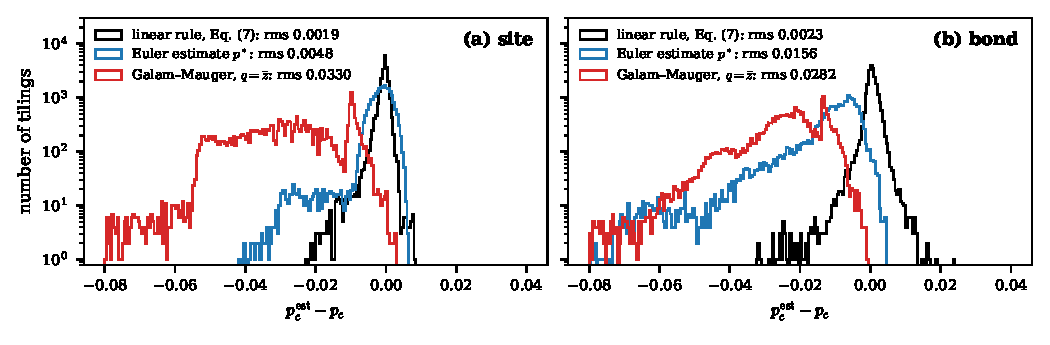
\includegraphics[width=\textwidth]{figs/fig_formulas.pdf}
\caption{Distribution of the errors of empirical estimates over the 23\,153 hold-out tilings with $k\ge5$: (a) site, (b) bond. Black: linear rule, Eq.~\eqref{eq:mix}, fitted on $k\le4$; blue: Euler-characteristic estimate $p^\ast$ of Ref.~\cite{Neher08}; red: Galam--Mauger formula~\cite{GalamMauger96} at $q=\zb$ (a few values below $-0.08$ are not shown).}
\label{fig:formulas}
\end{figure*}

\begin{table*}
\caption{Coefficients $\beta_t$ of the linear rule, Eq.~\eqref{eq:mix}: fit on the 243 tilings with $k\le4$ (used for all hold-out results) and, for reference, fit on all 23\,396 tilings. Standard errors from the residual scatter of the unweighted least-squares fit are given in parentheses. Also listed: the number of tilings that contain the vertex type, with $k\le4$ and in total, and the Archimedean thresholds $\pc(t)$ where they exist.}
\label{tab:beta}
\begin{ruledtabular}
\begin{tabular}{lrrllllll}
 & \multicolumn{2}{c}{tilings} & \multicolumn{3}{c}{site} & \multicolumn{3}{c}{bond}\\
type & $k\le4$ & all & $\beta$ ($k\le4$) & $\beta$ (all) & $\ps(t)$ & $\beta$ ($k\le4$) & $\beta$ (all) & $\pb(t)$\\
\hline
$(3^6)$ & 100 & 14286 & 0.5026(7) & 0.5041(2) & 0.5000 & 0.3460(5) & 0.3443(2) & 0.3473 \\
$(3^4.6)$ & 56 & 9903 & 0.5818(6) & 0.5827(1) & 0.5795 & 0.4334(8) & 0.4336(1) & 0.4343 \\
$(3^3.4^2)$ & 86 & 13338 & 0.5505(4) & 0.5508(1) & 0.5502 & 0.4190(4) & 0.4187(1) & 0.4196 \\
$(3^2.4.3.4)$ & 43 & 2086 & 0.5519(8) & 0.5525(2) & 0.5508 & 0.413(1) & 0.4134(2) & 0.4141 \\
$(3^2.4.12)$ & 16 & 666 & 0.716(4) & 0.721(1) &  & 0.596(6) & 0.598(2) &  \\
$(3^2.6^2)$ & 62 & 8476 & 0.656(1) & 0.6539(2) &  & 0.546(1) & 0.5453(2) &  \\
$(3.4.3.12)$ & 12 & 367 & 0.722(10) & 0.723(2) &  & 0.596(14) & 0.590(3) &  \\
$(3.4^2.6)$ & 64 & 12524 & 0.6235(6) & 0.6232(1) &  & 0.5181(6) & 0.5164(2) &  \\
$(3.4.6.4)$ & 36 & 1548 & 0.624(1) & 0.6249(3) & 0.6218 & 0.524(2) & 0.5235(3) & 0.5248 \\
$(3.6.3.6)$ & 76 & 14022 & 0.6502(9) & 0.6521(1) & 0.6527 & 0.5228(9) & 0.5230(2) & 0.5244 \\
$(3.12^2)$ & 12 & 335 & 0.819(15) & 0.831(3) & 0.8079 & 0.759(21) & 0.772(3) & 0.7404 \\
$(4^4)$ & 62 & 12636 & 0.5929(3) & 0.5929(1) & 0.5927 & 0.4980(6) & 0.4982(2) & 0.5000 \\
$(4.6.12)$ & 10 & 381 & 0.757(4) & 0.764(2) & 0.7478 & 0.703(5) & 0.712(1) & 0.6937 \\
$(4.8^2)$ & 1 & 1 & 0.7297$^\ast$ & 0.7297$^\ast$ & 0.7297 & 0.6768$^\ast$ & 0.6768$^\ast$ & 0.6768 \\
$(6^3)$ & 29 & 2146 & 0.701(2) & 0.7058(4) & 0.6970 & 0.655(2) & 0.6560(6) & 0.6527 \\

\end{tabular}
\end{ruledtabular}
\end{table*}

\subsection{Composition and arrangement}

The composition rules leave an rms error of about $2\times10^{-3}$, 30 to 100 times the statistical uncertainty of the atlas. Part of this error is due to the arrangement of the vertices, which a composition rule cannot see. The 23\,396 tilings have 6789 distinct compositions; 3287 of them are shared by two or more tilings (19\,894 tilings in total). For many groups the spread of the thresholds is within the statistical errors (median spread 1.9 combined standard errors for site and 3.2 for bond percolation). The spread exceeds five combined standard errors in 16\% (site) and 37\% (bond) of the groups; in these groups its median is $1.0\times10^{-3}$ (site) and $0.9\times10^{-3}$ (bond), and its maximum is $5.9\times10^{-3}$ and $2.3\times10^{-2}$. The largest spreads, in particular for bond percolation, occur for mixtures of $(6^3)$, $(3^2.6^2)$, $(3^4.6)$, and $(3^6)$ vertices, where the honeycomb and triangular regions can be arranged as compact domains or as thin interleaved stripes. Thus composition fixes $\pc$ only to about $10^{-3}$, and the arrangement can shift it by up to almost four orders of magnitude more than the uncertainty of the core values. The groups are listed in the Supplemental Material~\cite{SM}.

%=====================================================================
\section{Slip pairs}\label{sec:slip}
%=====================================================================

The smallest change of arrangement is a slip: two tilings that share the unit cell content and the first translation $\mathbf T_1$, while $\mathbf T_2'=\mathbf T_2\pm\mathbf T_1/2$. Such tilings consist of the same strips, stacked with different registry. Among the tilings with $k\le6$ there are 299 slip pairs (we restricted the census to $k\le6$; the list is in the Supplemental Material~\cite{SM}). Their site thresholds differ by more than five standard errors in 11\% of the pairs and their bond thresholds in 41\%. In all 34 pairs where both differences are resolved at this level, they have the same sign; the family below shows, however, that the site and bond differences can have opposite signs when the strips are far apart. Since many slip differences are unresolved, one may ask whether $\pc$ is exactly invariant under a slip for some pairs, for instance through an isomorphism of the matching graphs.

\begin{figure*}
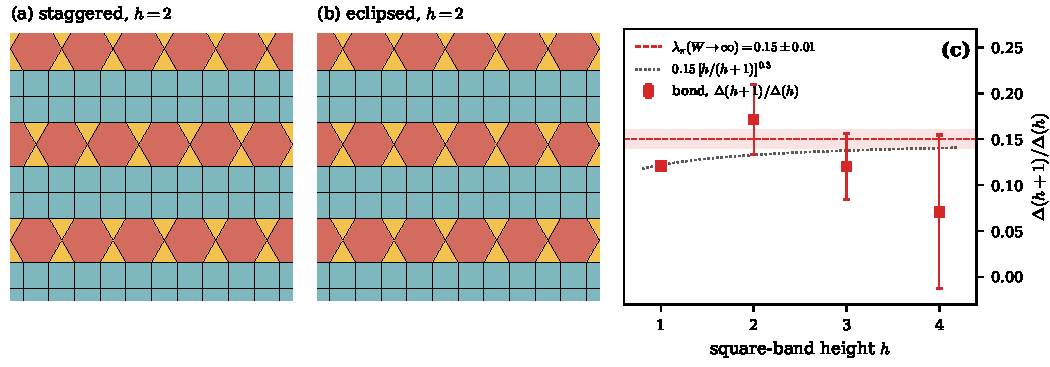
\includegraphics[width=\textwidth]{figs/fig_slip.pdf}
\caption{(a), (b) The staggered and eclipsed tilings of the slip family with $h=2$ rows of squares between the strips of hexagons and triangles; both have the composition $\tfrac47(3.4^2.6)+\tfrac27(4^4)+\tfrac17(3.6.3.6)$. (c) Threshold difference $\Delta=\pc(\text{eclipsed})-\pc(\text{staggered})$ as a function of $h$; filled symbols $\Delta>0$, open symbols $\Delta<0$, arrows: $2\sigma$ upper limits on $|\Delta|$ for unresolved differences. Dashed line and band: $A\lambda_\pi^{h}$ as in Eq.~\eqref{eq:tm}, with the amplitude $A$ fixed by $\Delta(1)$ and the leading $\kappa=\pi$ eigenvalue of the square-band transfer matrix extrapolated to infinite circumference, $\lambda_\pi=0.15\pm0.01$ (Appendix~\ref{app:tm}).}
\label{fig:slip}
\end{figure*}

\subsection{Is a threshold ever invariant under a slip?}

We found no evidence for exact invariance. The two-uniform pair already shows that a slip changes the site threshold: the difference is $2.73(5)\times10^{-4}$, i.e., $51\sigma$. Consistently, we found no isomorphism of the matching graphs that maps the translation lattice of one tiling onto that of the other: for every index from 4 to 8, the sets of quotients of the two matching graphs by all translation sublattices of that index differ (compared with \texttt{nauty}~\cite{McKayPiperno14}). Exact enumeration on small tori is not a useful test. On tori one period wide along $\mathbf T_1$ the two members of a slip pair give identical site polynomials $P_+(p)-P_0(p)$, and for another pair of four-uniform tilings with the same composition the polynomials coincide on all tori we enumerated, although the site and bond thresholds differ by $13\sigma$ and $11\sigma$. Whether some slip pair has exactly equal thresholds therefore remains open; in the family below the differences decay exponentially with the distance between the strips, so that unresolved differences are expected even without an exact symmetry.

\subsection{A clean family}

\begin{table}
\caption{Slip family of Fig.~\ref{fig:slip}: threshold difference $\Delta=\pc(\text{eclipsed})-\pc(\text{staggered})$ in units of $10^{-6}$. For $h=1$ and 4, and for bond percolation at all $h$, the values are differences of the extrapolated core thresholds. For site percolation at $h=2$ and 3 the difference was measured directly on identical tori ($24\times12$ and $25\times10$ unit cells, $10^9$ samples per tiling); there the finite-size bias largely cancels between the two members, but it is not controlled separately.}
\label{tab:slip}
\begin{ruledtabular}
\begin{tabular}{rlrr}
$h$ & $k$-uniform & $\Delta_{\rm site}$ & $\Delta_{\rm bond}$\\
\hline
1 & 2 & $+273(5)$ & $+1218(4)$\\
2 & 3 & $-11.5(1.0)$ & $+147(4)$\\
3 & 3 & $+0.5(1.0)$ & $+25(6)$\\
4 & 4 & $-4(6)$ & $+6(5)$\\
\end{tabular}
\end{ruledtabular}
\end{table}

To see how the effect of a slip depends on geometry, consider the family of Fig.~\ref{fig:slip}: strips of hexagons and triangle pairs (vertex types $(3.6.3.6)$ inside, $(3.4^2.6)$ on the boundary) separated by bands of $h$ rows of squares, with $(4^4)$ vertices inside the band. The strips have period $|\mathbf T_1|=2$ along their length. In the eclipsed member, consecutive strips are related by a translation perpendicular to them; in the staggered member they are shifted by half a period, one edge length. For $h=1$ the two members are the two two-uniform tilings with composition $\tfrac45(3.4^2.6)+\tfrac15(3.6.3.6)$; for $h=2,3$ they are three-uniform and for $h=4$ four-uniform. Table~\ref{tab:slip} and Fig.~\ref{fig:slip}(c) show the differences. The bond difference decreases by about an order of magnitude per row of squares, with ratios $\Delta(h+1)/\Delta(h)=0.121(3)$ and $0.17(4)$. The site difference decreases even faster and changes sign: $\Delta(2)/\Delta(1)=-0.042(4)$, and $\Delta(3)$ and $\Delta(4)$ are not resolved.

\subsection{A transfer-matrix hypothesis}

The slip changes only the relative registry of the strips. Consider the transfer matrix $\mathsf T$ that propagates the connectivity state of a row of the square band by one row (Appendix~\ref{app:tm}). It commutes with the shift $\mathsf S$ by one lattice spacing along the row, so its eigenvectors carry a momentum $\kappa$. A strip acts on the band as a boundary condition with period 2 along the row, i.e., with components in the sectors $\kappa=0$ and $\kappa=\pi$ only. Shifting one strip by one lattice spacing leaves the $\kappa=0$ component unchanged and reverses the sign of the $\kappa=\pi$ component. To first order in the coupling between the strips, the threshold difference is therefore carried by the propagation of the $\kappa=\pi$ component through the band,
\begin{equation}
\Delta(h)\simeq\sum_i A_i\lambda_{\pi,i}^{\,h},
\label{eq:tm}
\end{equation}
where $\lambda_{\pi,i}$ are the eigenvalues of $\mathsf T$ in the $\kappa=\pi$ sector and the amplitudes $A_i$ depend on the strips. The band itself is slightly supercritical at the thresholds of the tilings ($p=0.51$ for bond and $0.62$ for site percolation, above the square-lattice thresholds), and the eigenvalues depend only weakly on $p$ (Appendix~\ref{app:tm}). Long-wavelength fluctuations live in the sector $\kappa\to0$; in the $\kappa=\pi$ sector, which describes a modulation on the lattice scale, all eigenvalues we computed are small, $|\lambda_\pi|<0.15$, so $\Delta$ decays exponentially with $h$.

For bond percolation at $p=0.51$, the leading $\kappa=\pi$ eigenvalue on a cylinder of circumference $W$ is $\lambda_\pi=0.088$, 0.104, 0.115, 0.123, and 0.129 for $W=4$ to 12 (Table~\ref{tab:tm}). The increments decrease geometrically (ratio $\approx0.75$), and extrapolations in $1/W$, $1/W^2$, or by a geometric tail give $\lambda_\pi(W\to\infty)=0.15\pm0.01$. The leading eigenvalue has a nearly degenerate partner (0.128 at $W=12$), and further $\kappa=\pi$ eigenvalues follow at 0.090 and 0.074. The measured ratios, 0.121(3) for $h=1\to2$ and 0.17(4) for $h=2\to3$, are thus consistent in magnitude with $\lambda_\pi$. A weighted fit $\Delta(h)=A\lambda^h$ to all four bond values gives $\lambda=0.122(3)$ ($\chi^2=2.2$ for two degrees of freedom), dominated by $h=1$ and 2; without $h=1$ it gives $\lambda=0.18$ (68\% interval 0.14--0.21), in agreement with $\lambda_\pi=0.15\pm0.01$. More values at larger $h$ would be needed to determine the asymptotic rate from the data alone. The first ratio lies below the extrapolated $\lambda_\pi$; a ratio that increases toward $\lambda_\pi$ with $h$ is what Eq.~\eqref{eq:tm} gives when subleading modes contribute with the same sign at small $h$, but our data at $h\ge3$ are not precise enough to test this. For site percolation at $p=0.62$, the $\kappa=\pi$ sector contains positive and negative eigenvalues of similar magnitude: for $W=10$, $0.082$, $0.059$, $0.054$, and a twofold $-0.048$. A sign change of $\Delta$ is therefore allowed, and the measured ratio $-0.042(4)$ is consistent with a dominant contribution of the negative modes. With only two resolved values, however, the amplitudes cannot be determined independently, so the site data are consistent with Eq.~\eqref{eq:tm} but do not test it.

These observations suggest the following conjecture. Consider tilings composed of fixed strips separated by bands of $h$ rows of a periodic lattice, and two registries of the strips that differ by a shift of momentum $\kappa_0$. Then $\lim_{h\to\infty}h^{-1}\ln|\Delta\pc(h)|=\ln|\lambda|$, where $\lambda$ is the eigenvalue of largest modulus of the infinite-circumference band transfer matrix in the sector $\kappa_0$ that has a nonzero amplitude, evaluated at the limiting threshold of the family. For the square band and $\kappa_0=\pi$ this predicts that the bond difference eventually falls by a factor of about 7 per row. The conjecture can be tested on families with larger $h$ and on other strip types, which would also check that the rate does not depend on the strips. A proof would require control of the critical model on the whole tiling beyond the first-order argument above.

\begin{table}
\caption{Leading eigenvalues in the $\kappa=\pi$ sector of the transfer matrix of a square band of circumference $W$ (Appendix~\ref{app:tm}); bond at $p=0.51$, site at $p=0.62$. ``States'' is the number of non-crossing connectivity states.}
\label{tab:tm}
\begin{ruledtabular}
\begin{tabular}{rrlrl}
 & \multicolumn{2}{c}{bond} & \multicolumn{2}{c}{site}\\
$W$ & states & $\lambda_{\pi,i}$ & states & $\lambda_{\pi,i}$\\
\hline
4 & 14 & 0.0883, 0.0879 & 51 & 0.0555\\
6 & 132 & 0.1037, 0.1029, 0.0285 & 731 & 0.0685, $-0.0189$, $-0.0131$\\
8 & 1430 & 0.1148, 0.1138, 0.0760 & 12235 & 0.0770, 0.0501, 0.0484, $-0.0360$, $-0.0352$\\
10 & 16796 & 0.1230, 0.1219, 0.0828 & 223191 & 0.0817, 0.0588, 0.0539, $-0.0476$ (twofold)\\
12 & 208012 & 0.1292, 0.1280, 0.0896 & & \\
\end{tabular}
\end{ruledtabular}
\end{table}

%=====================================================================
\section{Conclusions}\label{sec:concl}
%=====================================================================

We have computed the site and bond percolation thresholds of all 23\,396 $k$-uniform tilings with $k\le10$. For $k\le4$ the values have uncertainties of a few units in the sixth decimal and are validated against all 22 Archimedean reference values; to our knowledge, they include the first thresholds of the 61 three-uniform and 151 four-uniform tilings and the first published bond thresholds of the two-uniform lattices, and they revise one two-uniform site threshold. The estimator based on the equality of the no-wrapping and cross-wrapping probabilities requires no knowledge of the torus anisotropy and is therefore suited to lattices of low symmetry. For the atlas values for $k=5$--10, a direct check on 200 thresholds, including the tilings with the largest cells and the most elongated tori, bounds the finite-size bias well below their statistical errors.

On the hold-out tilings, rules based on the vertex composition alone predict the threshold to about $2\times10^{-3}$, several times more accurately than the formulas we tested~\cite{GalamMauger96,Neher08,Lebrecht21,GalamMauger98}. Beyond this level the arrangement matters, by up to $2\times10^{-2}$ for bond percolation. For the smallest arrangement change, a slip of strips, the bond difference decays exponentially with the distance between the strips, at a rate consistent in magnitude with the momentum-$\pi$ sector of the band transfer matrix; we formulate the relation as a conjecture, which the present four values of $h$ do not yet test quantitatively.

The data invite several extensions. Critical polynomials computed by transfer matrices~\cite{Jacobsen14,ScullardJacobsen20} could improve the core values by several digits and provide high-precision site thresholds of lattices with several vertex orbits, which are still missing as references. Tilings composed of squares and triangles only, which approach dodecagonal quasicrystals~\cite{OxborrowHenley93}, could be followed to large $k$ and compared with the thresholds of quasiperiodic tilings~\cite{Babalievski95,ZiffBabalievski99}. The same lattices could also serve as test cases for the Potts model, where the corresponding wrapping identity contains the factor $q$~\cite{Arguin02,JacobsenScullard13}.

\begin{acknowledgments}
This research received no external funding. The author declares no competing interests. The author chose the research problem, directed the work and the computations, decided on the scope of the results and on their presentation, checked the results, and takes full responsibility for the content of the article. The large language model Claude Opus~5.5 (Anthropic) was employed under the strict control of the author and within a limited scope set by the author. Within this scope it was used to draft and edit the computer code for the computations and the text of the manuscript, to speed up the work.
\end{acknowledgments}

\section*{Data availability}
The thresholds of all 23\,396 tilings, with their uncertainties, compositions, torus data, and the periodic graphs, as well as the lists of slip pairs and composition groups and the results of the atlas finite-size check, are provided in the Supplemental Material~\cite{SM}. The periodic graphs are derived from the catalog snapshot of Ref.~\cite{TesCatalog} (commit 6772c7c6). The source code will be made openly available in a public repository [URL to be added].

\appendix

%=====================================================================
\section{Transfer matrix of the square band}\label{app:tm}
%=====================================================================

The band is a cylinder of the square lattice with circumference $W$ (even, to accommodate the period-2 boundary). The state of a row is a partition of its $W$ sites according to connectivity through the part of the band already traversed; for site percolation the state also records which sites are occupied, and only occupied sites carry connectivity labels. Since the traversed part of the band is topologically a disk bounded by the current row, only partitions that are non-crossing in the cyclic order occur; the numbers of such states are the Catalan numbers $C_W$ for bond percolation. One step of $\mathsf T$ adds a row of squares: first the vertical links to the new row (bond: each present with probability $p$; site: each new site occupied with probability $p$), then the horizontal links within the new row (bond: each present with probability $p$; site: present between occupied neighbors). For bond percolation this is the connectivity transfer matrix of the $q\to1$ Potts model~\cite{TemperleyLieb71,JacobsenScullard13}. We first computed the spectra in the basis of all set partitions; since $\mathsf T$ maps non-crossing states to non-crossing states, the matrix is block-triangular in that basis, and the spectrum of the non-crossing block (Table~\ref{tab:tm}) coincides, to all digits shown, with the leading eigenvalues found in the full basis for $W\le10$. The matrix is column-stochastic, so its largest eigenvalue in the $\kappa=0$ sector is 1. Since $\mathsf T$ commutes with the shift $\mathsf S$, the projector $\frac1W\sum_j e^{-i\kappa j}\mathsf S^j$ onto momentum $\kappa$ commutes with $\mathsf T$, and the eigenvalues in the $\kappa=\pi$ sector are obtained by the Arnoldi method applied to $\mathsf T$ times this projector. The values of $p$, 0.51 (bond) and 0.62 (site), are close to the thresholds of the $h=1$ tilings. At $W=8$, changing $p$ by $\pm0.02$ changes the bond eigenvalues by less than $0.002$ and the site eigenvalues by about 6\%.

%=====================================================================
\section{Three-uniform tilings}\label{app:tab}
%=====================================================================

Tables~\ref{tab:3uni} and \ref{tab:3unib} list the thresholds of the 61 three-uniform tilings. The identifier is the name of the file in the catalog of Ref.~\cite{TesCatalog}; it encodes the vertex orbits.

\begin{table*}
\caption{Site and bond thresholds of the 61 three-uniform tilings, ordered by decreasing site threshold (continued in Table~\ref{tab:3unib}). ID: catalog file name~\cite{TesCatalog}; $\zb$: mean degree.}
\label{tab:3uni}
\footnotesize
\begin{ruledtabular}
\begin{tabular}{rllrll}
 & ID & vertex types & $\zb$ & $\ps$ & $\pb$\\
\hline
1 & \texttt{3a 4a 4c 1} & $2/5\,(3^{2}.4.12)+2/5\,(3.4.3.12)+1/5\,(3.12^{2})$ & 3.800 & 0.7297711(25) & 0.6190292(27) \\
2 & \texttt{3a 4c 4l 1} & $1/2\,(3.4.3.12)+1/4\,(3.12^{2})+1/4\,(3.4.6.4)$ & 3.750 & 0.7255320(27) & 0.6224234(29) \\
3 & \texttt{3a 4a 4l 1} & $1/2\,(3^{2}.4.12)+1/4\,(3.12^{2})+1/4\,(3.4.6.4)$ & 3.750 & 0.7243694(26) & 0.6300425(30) \\
4 & \texttt{3c 4a 6d 1} & $6/13\,(3^{2}.4.12)+6/13\,(4.6.12)+1/13\,(3^{6})$ & 3.692 & 0.7166544(38) & 0.6336893(33) \\
5 & \texttt{3c 4h 4k 1} & $2/5\,(3.4^{2}.6)+2/5\,(4.6.12)+1/5\,(3.6.3.6)$ & 3.600 & 0.6857748(35) & 0.5911238(28) \\
6 & \texttt{3f 4d 4f 1} & $2/5\,(3^{2}.6^{2})+2/5\,(6^{3})+1/5\,(3.6.3.6)$ & 3.600 & 0.6697939(32) & 0.5821763(27) \\
7 & \texttt{3f 4d 4h 1} & $1/3\,(3^{2}.6^{2})+1/3\,(3.6.3.6)+1/3\,(6^{3})$ & 3.667 & 0.6671122(33) & 0.5713593(27) \\
8 & \texttt{4d 4g 4h 1} & $2/3\,(3.6.3.6)+1/3\,(3^{2}.6^{2})$ & 4.000 & 0.6512046(38) & 0.5300788(34) \\
9 & \texttt{3d 4d 6a 1} & $2/3\,(3^{2}.6^{2})+2/9\,(6^{3})+1/9\,(3^{6})$ & 4.000 & 0.6511325(36) & 0.5544924(30) \\
10 & \texttt{3f 4d 5a 1} & $1/3\,(3^{4}.6)+1/3\,(3^{2}.6^{2})+1/3\,(6^{3})$ & 4.000 & 0.6459708(61) & 0.5417084(45) \\
11 & \texttt{4a 4m 5c 1} & $2/5\,(3^{2}.4.12)+2/5\,(3.4.6.4)+1/5\,(3^{3}.4^{2})$ & 4.200 & 0.6437793(39) & 0.5305853(32) \\
12 & \texttt{4g 4h 4k 2} & $1/2\,(3.4^{2}.6)+1/2\,(3.6.3.6)$ & 4.000 & 0.6376763(50) & 0.5210539(43) \\
13 & \texttt{4g 4h 4k 1} & $1/2\,(3.4^{2}.6)+1/2\,(3.6.3.6)$ & 4.000 & 0.6375194(53) & 0.5202821(43) \\
14 & \texttt{4a 5e 6f 1} & $4/7\,(3^{2}.4.12)+2/7\,(3^{2}.4.3.4)+1/7\,(3^{6})$ & 4.571 & 0.6373104(53) & 0.4985799(34) \\
15 & \texttt{4d 4h 4k 2} & $1/2\,(3.4^{2}.6)+1/4\,(3^{2}.6^{2})+1/4\,(3.6.3.6)$ & 4.000 & 0.6363470(25) & 0.5253072(24) \\
16 & \texttt{4d 4h 4k 1} & $1/2\,(3.4^{2}.6)+1/4\,(3^{2}.6^{2})+1/4\,(3.6.3.6)$ & 4.000 & 0.6361815(64) & 0.5244735(27) \\
17 & \texttt{4h 4k2 6} & $4/5\,(3.4^{2}.6)+1/5\,(3.6.3.6)$ & 4.000 & 0.6282443(34) & 0.5182987(29) \\
18 & \texttt{4a 5c 6i 1} & $1/2\,(3^{2}.4.12)+1/4\,(3^{6})+1/4\,(3^{3}.4^{2})$ & 4.750 & 0.6240755(55) & 0.4872769(34) \\
19 & \texttt{4k 4l2 1} & $1/2\,(3.4^{2}.6)+1/2\,(3.4.6.4)$ & 4.000 & 0.6218128(35) & 0.5205844(30) \\
20 & \texttt{4e 4k 5c 1} & $2/5\,(3^{2}.6^{2})+2/5\,(3.4^{2}.6)+1/5\,(3^{3}.4^{2})$ & 4.200 & 0.6210445(52) & 0.5094462(44) \\
21 & \texttt{4f 4k 4r 1} & $4/7\,(3.4^{2}.6)+2/7\,(4^{4})+1/7\,(3.6.3.6)$ & 4.000 & 0.6183577(32) & 0.5130626(27) \\
22 & \texttt{4f 4k 4s 1} & $4/7\,(3.4^{2}.6)+2/7\,(4^{4})+1/7\,(3.6.3.6)$ & 4.000 & 0.6183478(32) & 0.5132098(27) \\
23 & \texttt{4k 4l 4o 1} & $4/7\,(3.4^{2}.6)+2/7\,(3.4.6.4)+1/7\,(4^{4})$ & 4.000 & 0.6176267(18) & 0.5159154(16) \\
24 & \texttt{4f 4k 4u 1} & $4/9\,(3.4^{2}.6)+4/9\,(4^{4})+1/9\,(3.6.3.6)$ & 4.000 & 0.6128031(37) & 0.5102344(32) \\
25 & \texttt{4f 4k 4u 2} & $4/9\,(3.4^{2}.6)+4/9\,(4^{4})+1/9\,(3.6.3.6)$ & 4.000 & 0.6127977(61) & 0.5102596(46) \\
26 & \texttt{4h 5a 6a 1} & $6/13\,(3^{4}.6)+6/13\,(3.6.3.6)+1/13\,(3^{6})$ & 4.615 & 0.6105655(18) & 0.4729273(17) \\
27 & \texttt{4k 4l 5e 1} & $1/2\,(3.4^{2}.6)+1/4\,(3^{2}.4.3.4)+1/4\,(3.4.6.4)$ & 4.250 & 0.6055637(17) & 0.4914115(16) \\
28 & \texttt{4d 5a 6f 1} & $2/5\,(3^{4}.6)+2/5\,(3^{2}.6^{2})+1/5\,(3^{6})$ & 4.800 & 0.5969555(24) & 0.4605932(35) \\
29 & \texttt{4e 5b 6i 3} & $2/5\,(3^{4}.6)+2/5\,(3^{2}.6^{2})+1/5\,(3^{6})$ & 4.800 & 0.5962765(57) & 0.4592692(45) \\
30 & \texttt{4f 5a 6a 1} & $3/5\,(3^{4}.6)+3/10\,(3.6.3.6)+1/10\,(3^{6})$ & 4.800 & 0.5957901(49) & 0.4548427(30) \\
31 & \texttt{4k 5e 6a 1} & $12/19\,(3.4^{2}.6)+6/19\,(3^{2}.4.3.4)+1/19\,(3^{6})$ & 4.421 & 0.5957781(38) & 0.4761811(28) \\

\end{tabular}
\end{ruledtabular}
\end{table*}

\begin{table*}
\caption{Continuation of Table~\ref{tab:3uni}.}
\label{tab:3unib}
\footnotesize
\begin{ruledtabular}
\begin{tabular}{rllrll}
 & ID & vertex types & $\zb$ & $\ps$ & $\pb$\\
\hline
32 & \texttt{4g 5b2 1} & $4/5\,(3^{4}.6)+1/5\,(3.6.3.6)$ & 4.800 & 0.5951624(36) & 0.4532446(29) \\
33 & \texttt{4m 5e 6a 1} & $12/19\,(3.4.6.4)+6/19\,(3^{2}.4.3.4)+1/19\,(3^{6})$ & 4.421 & 0.5951617(40) & 0.4785771(27) \\
34 & \texttt{4i 5b2 1} & $4/5\,(3^{4}.6)+1/5\,(3.6.3.6)$ & 4.800 & 0.5951600(54) & 0.4532491(41) \\
35 & \texttt{4k 5a 5c 1} & $1/2\,(3.4^{2}.6)+1/4\,(3^{4}.6)+1/4\,(3^{3}.4^{2})$ & 4.500 & 0.5949609(17) & 0.4734438(27) \\
36 & \texttt{4d 5a 6h 1} & $1/3\,(3^{6})+1/3\,(3^{4}.6)+1/3\,(3^{2}.6^{2})$ & 5.000 & 0.5826779(35) & 0.4420118(29) \\
37 & \texttt{4s2 5c 1} & $2/3\,(4^{4})+1/3\,(3^{3}.4^{2})$ & 4.333 & 0.5788109(29) & 0.4718739(21) \\
38 & \texttt{4p 4s 5c 1} & $3/5\,(4^{4})+2/5\,(3^{3}.4^{2})$ & 4.400 & 0.5759992(32) & 0.4664677(26) \\
39 & \texttt{4f 5b 6i 1} & $4/7\,(3^{4}.6)+2/7\,(3^{6})+1/7\,(3.6.3.6)$ & 5.143 & 0.5700176(69) & 0.4227173(26) \\
40 & \texttt{4l 5d 6d 1} & $3/5\,(3^{3}.4^{2})+3/10\,(3.4.6.4)+1/10\,(3^{6})$ & 4.800 & 0.5690721(39) & 0.4437350(27) \\
41 & \texttt{4l 5f 6d 1} & $3/5\,(3^{2}.4.3.4)+3/10\,(3.4.6.4)+1/10\,(3^{6})$ & 4.800 & 0.5689262(38) & 0.4371290(26) \\
42 & \texttt{5a 5b 6f 1} & $6/7\,(3^{4}.6)+1/7\,(3^{6})$ & 5.143 & 0.5687854(26) & 0.4213160(27) \\
43 & \texttt{4s 5c2 2} & $2/3\,(3^{3}.4^{2})+1/3\,(4^{4})$ & 4.667 & 0.5646654(26) & 0.4453207(22) \\
44 & \texttt{5a 5c 5e 1} & $1/3\,(3^{4}.6)+1/3\,(3^{3}.4^{2})+1/3\,(3^{2}.4.3.4)$ & 5.000 & 0.5601703(25) & 0.4224297(15) \\
45 & \texttt{4p 5c2 1} & $4/5\,(3^{3}.4^{2})+1/5\,(4^{4})$ & 4.800 & 0.5589115(32) & 0.4349439(24) \\
46 & \texttt{4s 5c 6f 1} & $2/5\,(3^{3}.4^{2})+2/5\,(4^{4})+1/5\,(3^{6})$ & 4.800 & 0.5583123(42) & 0.4348991(28) \\
47 & \texttt{4o 5d 5f 1} & $4/9\,(3^{3}.4^{2})+4/9\,(3^{2}.4.3.4)+1/9\,(4^{4})$ & 4.889 & 0.5552546(37) & 0.4248748(25) \\
48 & \texttt{5d 5f2 3} & $2/3\,(3^{2}.4.3.4)+1/3\,(3^{3}.4^{2})$ & 5.000 & 0.5505561(40) & 0.4155871(27) \\
49 & \texttt{5d2 5f 1} & $2/3\,(3^{3}.4^{2})+1/3\,(3^{2}.4.3.4)$ & 5.000 & 0.5503553(42) & 0.4173329(27) \\
50 & \texttt{4p 5c 6f 1} & $1/2\,(3^{3}.4^{2})+1/4\,(3^{6})+1/4\,(4^{4})$ & 5.000 & 0.5494188(38) & 0.4197311(26) \\
51 & \texttt{4s 5c 6i 1} & $1/3\,(3^{6})+1/3\,(3^{3}.4^{2})+1/3\,(4^{4})$ & 5.000 & 0.5491069(48) & 0.4197692(32) \\
52 & \texttt{5e2 6a 1} & $12/13\,(3^{2}.4.3.4)+1/13\,(3^{6})$ & 5.077 & 0.5471092(19) & 0.4085816(15) \\
53 & \texttt{5c 5e 6a 1} & $6/13\,(3^{3}.4^{2})+6/13\,(3^{2}.4.3.4)+1/13\,(3^{6})$ & 5.077 & 0.5466653(17) & 0.4102233(15) \\
54 & \texttt{5a 6c 6f 1} & $6/11\,(3^{4}.6)+5/11\,(3^{6})$ & 5.455 & 0.5444742(35) & 0.3931541(27) \\
55 & \texttt{5c2 6f 1} & $4/5\,(3^{3}.4^{2})+1/5\,(3^{6})$ & 5.200 & 0.5407132(35) & 0.4047014(26) \\
56 & \texttt{4p 5c 6i 1} & $2/5\,(3^{6})+2/5\,(3^{3}.4^{2})+1/5\,(4^{4})$ & 5.200 & 0.5399914(40) & 0.4048875(27) \\
57 & \texttt{5c2 6i 2} & $2/3\,(3^{3}.4^{2})+1/3\,(3^{6})$ & 5.333 & 0.5342092(33) & 0.3949105(27) \\
58 & \texttt{5a 6f 6i 1} & $3/5\,(3^{6})+2/5\,(3^{4}.6)$ & 5.600 & 0.5328439(34) & 0.3804784(26) \\
59 & \texttt{5b 6j2 1} & $2/3\,(3^{6})+1/3\,(3^{4}.6)$ & 5.667 & 0.5274497(34) & 0.3748076(25) \\
60 & \texttt{5c 6f 6i 1} & $3/5\,(3^{6})+2/5\,(3^{3}.4^{2})$ & 5.600 & 0.5209515(33) & 0.3756874(26) \\
61 & \texttt{5c 6i2 1} & $2/3\,(3^{6})+1/3\,(3^{3}.4^{2})$ & 5.667 & 0.5175410(38) & 0.3709436(26) \\

\end{tabular}
\end{ruledtabular}
\end{table*}

\clearpage
\bibliography{refs}

\end{document}
